\chapter{はじめに}
あああああああああああああああああああああああああああああああああああああああああああああああああああああああああああああああああああああああああああああああああああああああああああああああああああああああああああああああああああああああああああああああああああああああああああああああ

参考文献はこんな感じで引用します.
\cite{Quinlan96}
\cite{Quinlan89}
\cite{Quinlan93}
\cite{Iba94}
\cite{C50}
\cite{Nakayama00}
\cite{Otani06}
\cite{Otani04}
\cite{Saino88}
\cite{Ishibashi11}
\cite{Ushijima11}


図はこんな風に入れます.

\begin{figure}[tbhp]
\begin{center}
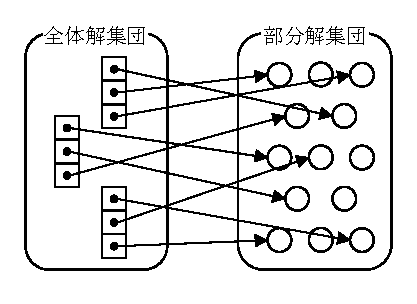
\includegraphics[scale=0.95]{images/se.eps}
\caption{共生進化における2つの集団}
\label{fig:02se}
\end{center}
\end{figure}

図番号は図\ref{fig:02se}のように参照します.
